
\documentclass[tikz,border=5pt]{standalone}
\usetikzlibrary{spath3}
\begin{document}
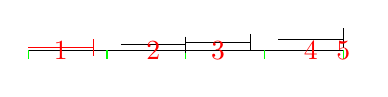
\begin{tikzpicture}
    \draw[spath/save=npath] (0,0) 
        foreach \k in {1,...,4} { -- ++(1,0) +(0,0)};
    \draw[green] (0,0) -- +(0,-3pt) 
        foreach \k in {1,...,4} { -- +(0,-3pt) ++(1,0)} -- +(0,-3pt);

    \tikzset{
        path 1/.style={red},
        spath/.cd,
        insert gaps after components={npath}{10pt}{1,3}, 
        get components of={npath}\components,
    }

    \foreach[count=\k] \cpt in \components {
        \path[ 
            draw,
            path \k/.try,
            spath/.cd, 
            translate=\cpt{0pt}{\k pt}, 
            use=\cpt,
        ] +(0,3pt) -- +(0,-3pt);
        \node[text=red] at (spath cs:{\cpt} .5) {\(\k\)};
    }
\end{tikzpicture}
\end{document}